
\newpage

\section{Data Collection and Measurement}
% Discuss the analytical methods used in the study.
% - Refer to relevant data tables.


\subsection{Field Sampling}
Both springs and rain were sampled in the field. Springs were sampled according to locations visited in past expeditions. Rain was collected in a rain gauge along several transects. Six aliquots were collected for each spring for anion, cation, titration, DIC, isotope and archive purposes. Both water bodies were measured in the field for temperature, pH and TDS on Hanna Instruments HI-991300 and EXTECH DO700. Samples were also titrated using a Hach digital titrator with 0.0625M HCl to calculate the alkalinity of the water following the Gran Method \parencite{gran1952}. Titrations were done on 50ml aliquots, 24 hours within having been collected.  Rain samples had a smaller yield and so only three aliquots were collected, for cation and anion, isotope and archive purposes. Both water body types were filtered through a 0.2$\micro$m PES membrane in a filtration unit prior to bottling. Cation and archive samples were acidified with concentrated HNO$_3$ to give a pH of $\sim$2, keeping the cations in solution. 


\subsection{Major and Trace Element Analysis}

Cation concentrations were determined using an Agilent Technologies 5100 Inductively-Coupled Plasma Optical Emission Spectrometer (ICP-OES) using a calibration line made from a Nepalese spring stock solution. Anion concentrations were determined using a Dionex Ion Chromatography System (ICS) 5000 series against the Battle-02 standard calibration line. Associated uncertainties range between 5-10\% for cations and anions.

%fact check the anion uncertainty

% \subsection{Isotope Analysis}

% Samples for radiogenic strontium analysis were dried down to provide at least 100 ng of Sr. Samples were then dissolved in aqua regia (3:1 HNO$_\text{3}$:HCl) to remove any additional organic matter. Once dried down again, they were added to 3 ml teflon columns with Eichrom SrSpec$^{\textcopyright}$ resin pipetted in. Once washed three times with Milli-Q$^{\textregistered}$ water, the column was primed with 3M HNO$_\text{3}$. The sample was centrifuged then loaded onto the column avoiding any solids. The column was then washed a total of three times with 3M HNO$_3$ to remove other cations. Lastly, the column was eluted to a beaker with Milli-Q$^{\textregistered}$ water to collect the Sr. Once dried, the samples were dissolved in 3M HNO$_\text{3}$, centrifuged and then diluted for analysis on a Thermo Scientific Neptune Plus MC-ICP-MS. Errors on Sr isotope measurement are taken from two standard deviations of the measured values given by the MC-ICP-MS.

% % \bsk

% Samples were also analysed for stable oxygen and deuterium isotopes on a Picarro L2140-i portable analyser, using cavity ring-down spectroscopy, with an average precision of 0.05, 0.09 and 0.57 \textperthousand\ for $\delta^{17}O$, $\delta^{18}O$ and $\delta D$ respectively. 


\newpage

\section{Methods and Models for Analysis}


\subsection{Rain and Hydrothermal Correction}

Rain input is a significant factor in the chemical composition of groundwater and rivers. Most chloride found in these water bodies is thought to be due to rainwater input \parencite{dreverGeochemistryNaturalWaters1997}. It is standard practice to correct for this input using the measured concentrations of chloride in the rain. Rain samples collected in the September 2024 season are used for this correction, detailed in Appendix 1. Once the samples have been corrected for rain input, the remaining chloride is assumed to be derived from hydrothermal signatures encountered in the flow path. Spring waters are also therefore corrected for hydrothermal input using the most chloride-rich springs, so that the concentrations used for modelling are strictly derived from weathering reactions.

\subsection{Identifying the Weathering Reaction}
\label{subsection:weathering}

The first step towards quantifying the extent to which chemical weathering reactions have gone to completion is to discern what reaction is taking place. In principle this is as simple as knowing what minerals are dissolving (the "forward" reaction) and which are precipitating (the "backward" reaction). Modal decomposition is a mathematical method that can be applied to consider several minerals that could be dissolving and/or precipitating, and how they contribute to the spring chemistry (\cite{garrelsOriginChemicalComposition1967}; \cite{dreverGeochemistryNaturalWaters1997}). Note that this calculation can only be done if the number of components is the same as, or greater than the number of minerals.


\begin{center}
\[
  \begin{bordermatrix}
{ & Biot & Plag & Calc & Smec & Kaol & KSpar \cr
Si  & a_{11}  & a_{12}  & a_{13}  & a_{14}  & a_{15}  & a_{16}  \cr
Al  & a_{21}  & a_{22}  & a_{23}  & a_{24}  & a_{25}  & a_{26}  \cr
Mg  & a_{31}  & a_{32}  & a_{33}  & a_{34}  & a_{35}  & a_{36}  \cr
Ca  & a_{41}  & a_{42}  & a_{43}  & a_{44}  & a_{45}  & a_{46}  \cr
Na  & a_{51}  & a_{52}  & a_{53}  & a_{54}  & a_{55}  & a_{56}  \cr
K   & a_{61}  & a_{62}  & a_{63}  & a_{64}  & a_{65}  & a_{66}  \cr}
  \end{bordermatrix}
  \cdot
  \begin{bordermatrix}
{ &  \cr
  & x_{Biot} \cr
  & x_{Plag} \cr
  & x_{Calc} \cr
  & x_{Smec} \cr
  & x_{Kaol} \cr
  & x_{KSpar} \cr}
  \end{bordermatrix}
  =
  \begin{bordermatrix}
{ & Spring (\mu mol/l) \cr
  & b_1 \cr
  & b_2 \cr
  & b_3 \cr
  & b_4 \cr
  & b_5 \cr
  & b_6 \cr}
  \end{bordermatrix}
\]
\end{center}
\bsk

Matrix algebra facilitates the calculations of the molar proportions of mineral added to the water. Given known matrices \( A \) and \( B \), where A represents the stoichiometric quantities of elements in a mineral, and B the concentrations of elements in the water:

\begin{equation}
AX = B
\end{equation}
\begin{equation}
X = A^{-1}B
\end{equation}

The matrix X, corresponding to molar proportions of mineral added to the water, can then be calculated, under the assumptions that all minerals dissolve in a congruent fashion. Modal decompostion for spring waters was performed according to stoichiometric proportions from \textcite{bickleDiscriminationCarbonateSilicate2015}.\\

\begin{figure}[h]
    \centering
    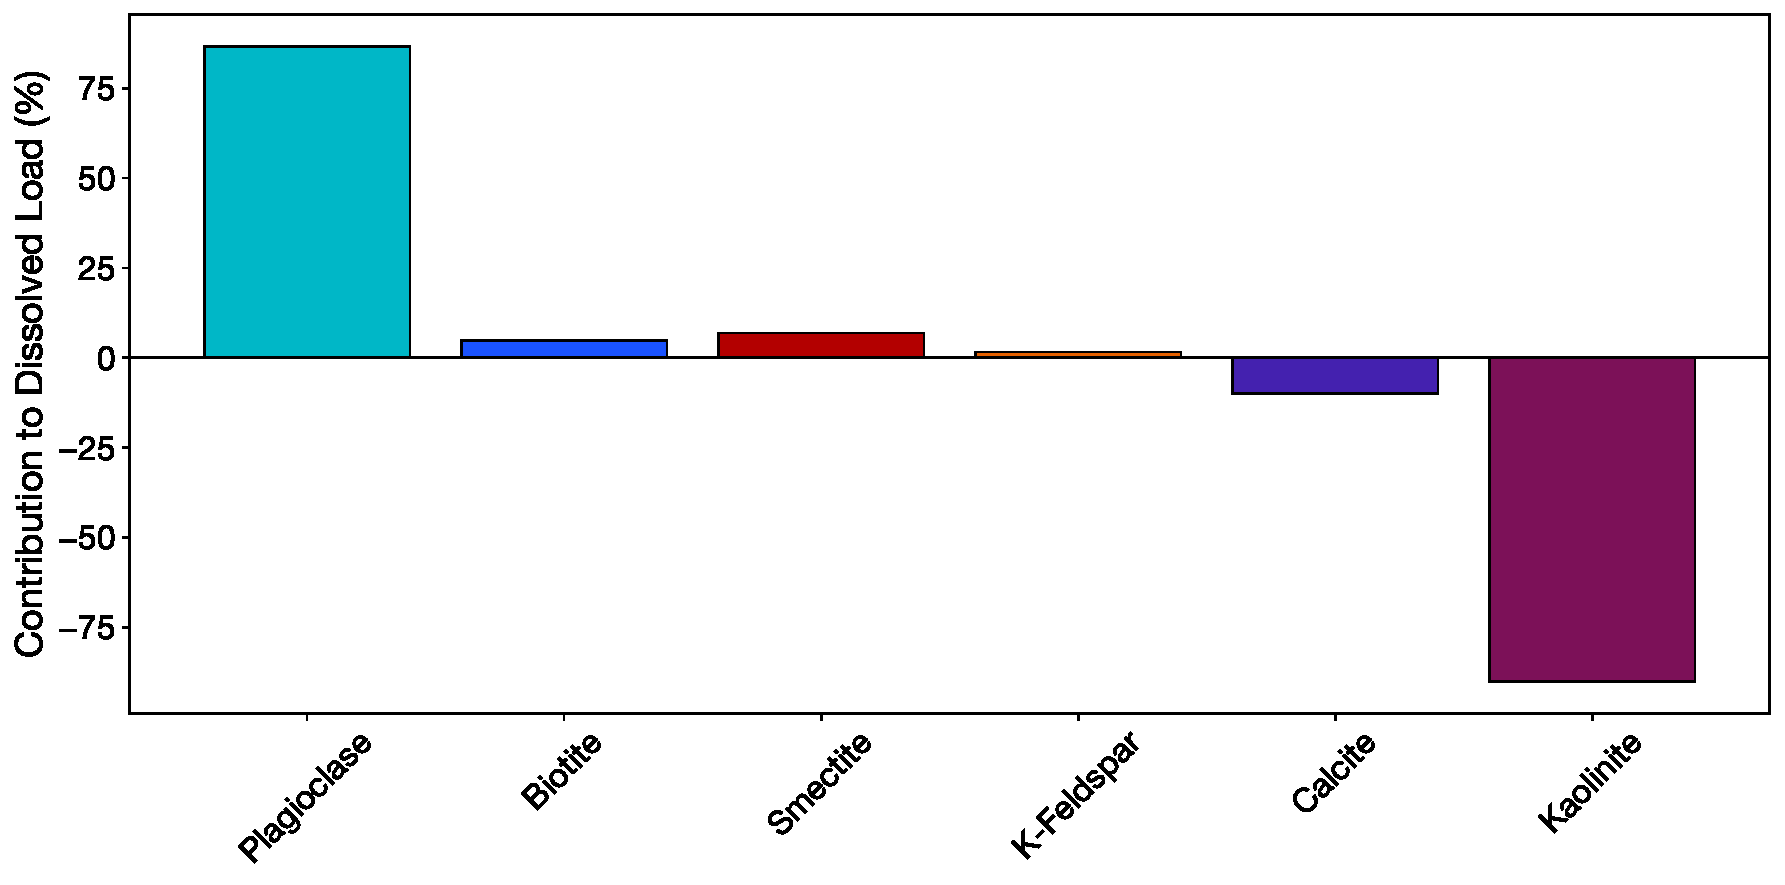
\includegraphics[width=\textwidth]{Normalized_Average_Mineral_Volume_Changes.pdf}
    \caption{Modal Decomposition results averaged over all springs. y-axis corresponds to modal proportion of mineral contributing to the dissolved (measured) load. Negative y-space indicates the mineral is involved in the backward reaction.}
    \label{fig:modal}
\end{figure}

\FloatBarrier

Figure \ref{fig:modal} suggests that the major phase being dissolved is plagioclase feldspar (the forward reaction) and the major phase being precipitated is kaolinite (the backward reaction). Plagioclase feldspar is made up of a solid solution of albite (NaAlSi$_3$O$_8$) and anorthite (CaAl$_2$Si$_2$O$_8$) \parencite{HENRY1982381}. A plagioclase with composition An$_x$ (or equivalently Ab$_y$) is made up of x mol \% anorthite and y mol \% albite. The primary composition of plagioclase in the area averages to $\approx$ An-20 with considerable scatter in the data (\cite{bickleDiscriminationCarbonateSilicate2015}; \cite{knightImpactAdsorptionDesorption2024}). The joint plagioclase to kaolinite reaction is given by the following equation (written so that aluminium is conserved):


\begin{equation}
    \small
    An_{20} + 1.2 H^{+}_{\text{(aq)}} + 0.6 H_{2}O \rightarrow
    0.6 \text{Kaolinite} + 0.8 Na^{+}_{\text{(aq)}} + 0.2 Ca^{2+}_{\text{(aq)}} + 1.6 SiO_{2 \text{(aq)}}
\label{eq:10}
\end{equation}
\quad Or
\begin{equation}
    \hspace{-0.3cm}
    \small
    Ca_{0.20}Na_{0.80}Al_{1.20}Si_{2.80}O_{8} + 1.2H^{+} + 0.6 H_{2}O \rightarrow 
    0.6 Al_{2}Si_{2}O_{5}(OH)_{4} + 0.8 Na^{+} + 0.2 Ca^{2+} + 1.6 SiO_{2}
    \label{eq:9}
\end{equation}



\subsection{One-Dimensional Reactive Transport Models}

Reactive transport models can be used to estimate the residence time of water in a catchment. These models are widely used in applied fluid dynamics and various fields within Earth Sciences. They aim to track chemical reactions occurring at each spatial point, accounting for the movement of reactants to and reaction products away from those points \parencite{bethkeGEOCHEMICALBIOGEOCHEMICALREACTION}. The basic form of a reactive transport model is a partial differential equation that describes the transport of solutes and the reactions that occur between them. For reacting solutes, concentration changes over time are governed by transport rates and the relative rates of dissolution and precipitation \parencite{bethkeGEOCHEMICALBIOGEOCHEMICALREACTION}.
These models simplify a real world three-dimensional catchment into one-dimensional flow paths. The proposed equations can be complex, but in simple cases a species of concentration $C_i$ can be modelled to follow a first-order rate law, generally represented by:

\begin{equation}
    \frac{\partial C_i}{\partial t} = \mathcal{O}_{T}(C_i) + \mathcal{O}_{R}(C_i)
    \label{eq:1}
\end{equation}


Where \(\mathcal{O}_{T}\) and \(\mathcal{O}_{R}\) are the transport and reaction operators, respectively \parencite{bethkeGEOCHEMICALBIOGEOCHEMICALREACTION}. Transport operators are derived from the divergence principle; this states that the rate of change in the concentration of a component over time depends on how the advective and dispersive fluxes vary spatially and temporally. Depending on the hypothesis supported, equation \ref{eq:1} can be modified accordingly. The following sections will discuss two models with their own versions of equation \ref{eq:1}.

\subsubsection*{The Role of Porosity and Permeability}

Estimation of porosity and permeability is essential for understanding the extent of weathering in a catchment. Understanding how open a rock is to water flow and reaction can constrain the reactive transport models used to estimate residence time. Porosities vary widely across a catchment depending on the rock type encountered (\cite{singhWeatheringPotentialIndex1987}; \cite{davidLaboratoryMeasurementCompactioninduced1994}). Porosity also increases as a rock becomes more weathered \parencite{marquesWeatheringZonesMetamorphic2010}. Note that in the following models, the porosity value is taken to be an average over a given depth in the subsurface. In Earth Sciences, models of fluid flow — whether in the subsurface or deep within the Earth — are typically categorized based on whether the flow occurs through a porous medium or within large open channels (\cite{pedrazasRelationshipTopographyBedrock2021}; \cite{maherRoleFluidResidence2011}; \cite{kelemenExtractionMidOceanRidge1995}; \cite{jacksonChemicalDifferentiationCold2018}). This remains an open debate beyond the scope of this study (though note that flow paths are depicted as "channels" to facilitate the explanation of reactive transport, see Figure \ref{fig:reactsketch}). Hence, the porosity value used for residence time calculation in the reactive transport models is assumed to be an average. This allows for both types of flow to be plausible, whether in a highly porous medium or large channels surrounded by less porous rock. Also note that these models do not directly consider permeability.

\subsubsection*{Model Motivation}

As discussed in the Introduction, there are different hypotheses regarding the major controls on chemical weathering. This study will contrast one model that assumes kinetic weathering rates are constant, with another which assumes the rates change with the amount of runoff and the approach to chemical equilibrium. These two, Fontorbe and Maher models, respectively follow different hypotheses regarding the strongest control on weathering as a result of their assumptions. The Fontorbe model exhibits greater sensitivity to temperature than the Maher model which is more influenced by runoff. The benchmark for a model's effectiveness will be how well it can predict residence times compared to previous studies on gas tracers. Assumptions and constraints will be compared and contrasted, and their results used to inform the calculation of rates of reaction and approach to equilibrium in Melamchi. For both models, the element used to estimate residence times is dissolved silicon (DSi). The element silicon is present in both dissolution and precipitation reactions, so it is applicable to the Maher model which considers both reactions. Furthermore, DSi is what both models were built for in their respective original studies. Lastly, both models use the same reaction rate constant $k$ = $10^{-15}$ mol m$^{-2}$ s$^{-1}$; this is considered a value appropriate to use for close to equilibrium settings.


\begin{figure}[h]
    \centering
    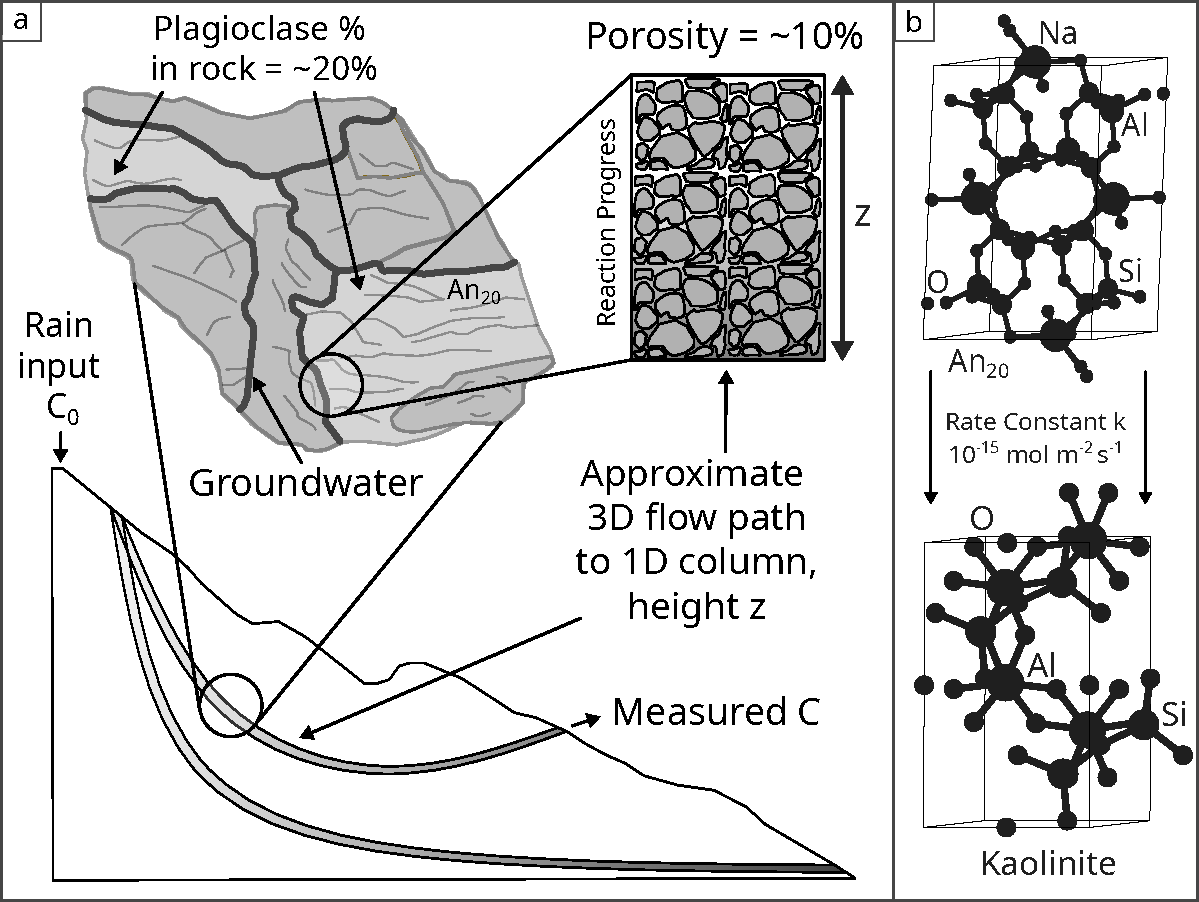
\includegraphics[width=\textwidth]{sketch.pdf}
    \caption{(a) Illustration showing workflow performed in reactive transport models. Sketch shows different parameters used, such as the rain input at the top of the catchment used for the initial "$C_0$" concentration, the plagioclase percentage in the rock as well as the porosity. (b) Mineral ball and spoke models showing the dissolution of plagioclase and precipitation of kaolinite. Ball and spoke models adapted from \textcite{vaitkusWorkflowDerivingChemical2023}, \textcite{grazulisComputingStoichiometricMolecular2015}, \textcite{downsAmericanMineralogistCrystal2003}.}
    \label{fig:reactsketch}
\end{figure}

\FloatBarrier

\newpage

\subsubsection*{\textcite{fontorbeSiliconIsotopicComposition2013} - Model Equations}

\textcite{fontorbeSiliconIsotopicComposition2013} investigates silicon isotopic composition in the Ganges River, assuming constant reaction rates along flow paths (see Appendix 2 for a full derivation, and Table \ref{tab:fontorbe1} for a list of parameters used). This model was initially constructed to reproduce DSi concentration and $\delta^{30}$Si in the Ganges, but is being repurposed in a novel fashion for this study. The first-order differential equation governing transport and reaction is given as:\\

    \begin{equation}
    \phi \frac{\partial C}{\partial t} = -\omega \phi \frac{\partial C}{\partial z} + R_n(1-f)
    \label{eq:fontorbe}
    \end{equation}\\

Where \( C \) is the elemental concentration in $\mu$mol/L, $\omega$ is the fluid velocity in m/s, $\phi$ is the rock porosity, z is a position along the flow path in m, R$_\text{n}$ is the rate of reaction in mol/m$^3$/s, and f is the fraction of Si present in the dissolved load that is reprecipitated in the back reaction. The equation can be nondimensionalised using the Damköhler number (\(N_D\)), which describes the relative importance of kinetic vs transport-controlled settings \parencite{bethkeGEOCHEMICALBIOGEOCHEMICALREACTION}:\\

\begin{equation}
    N_D = \frac{R_n h}{\phi C_0 \omega}
\end{equation}\\

Where h is the full length of the flow path (i.e. the maximum z). For a flow path averaged as stated above, the porosity is so small that the relative fractions of reacting phases do not change with time as much as the advective and transport terms. As such, the steady state (\(\partial C/\partial t = 0\)) assumption can be used and the concentration at the end of the flow path can be rearranged to give the residence time \(T_f\):\\

\begin{equation}
    T_f = \frac{(C - C_0)\phi}{(1-f)R_n}
\end{equation}


\begin{table}[H]
    \centering
    \renewcommand{\arraystretch}{1.1} % Adjust row height
    \begin{tabular}{|c|c|c|c|}
        \hline
        \multicolumn{4}{|c|}{\textbf{\textcite{fontorbeSiliconIsotopicComposition2013} - Model Parameters}} \\  
        \hline
        \textbf{Parameter} & \textbf{Definition} & \textbf{Units} & \textbf{Formula (Value)} \\  
        \hline
        $\phi$ & Porosity & - & 0.1 $^*$\\
        $\omega$ & Fluid velocity & m/s & Variable \\
        $h$ & Length of flow path & m & Variable \\
        $C$ & Concentration \@ end of flow path & $\mu$mol/L & Variable \\
        $C_0$ & Initial concentration & $\mu$mol/L & Rain Input \\
        $f$ & Fraction reprecipitated & - & 0.5$^*$ \\
        $N_D$ & Damkohler Number & - & $N_D = \frac{R_n h}{\phi C_0 \omega}$ \\
        $T_f$ & Residence time & s & $T_f = \frac{h}{\omega\phi}$ \\
        $R_n$ & Reaction rate & mol/m$^3$/s & $\rho \cdot 10^6 \cdot k \cdot S \cdot X $ \\
        $k$ & Dissolution rate constant & mol/m$^2$/s & 10$^{-15*}$ \\
        $S$ & Specific surface area & m$^2$/g & 0.1$^*$ \\
        $\rho$ & Plagioclase density & g/cm$^3$ & 2.7$^*$ \\
        $X$ & Volume fraction of mineral in rock & $g_{min}/g_{rock}$ & 0.2$^*$ \\
        \hline
    \end{tabular}
    \caption{Key parameters and definitions for the Fontorbe model. $^*$ - Values used for calculation.}
    \label{tab:fontorbe1}
\end{table}


\FloatBarrier


\newpage



\subsubsection*{\textcite{maherRoleFluidResidence2011} - Model Equations}

This model is built in accordance with the principle that the main control on silicate weathering is runoff. The model is based on the assumption that the reaction rate decreases linearly with approach to equilibrium, and that all weathering paths approach equilibrium. The model is initally set out in \textcite{maherRoleFluidResidence2011} and further developed in \textcite{maherHydrologicRegulationChemical2014}. The motivation behind the hydrological control on weathering is based on sensitivity analyses of real catchment data on one-dimensional reactive transport models which suggest that porosity, mineral surface area, and temperature have no consistent correlation with water composition \parencite{maherRoleFluidResidence2011}. See Appendix and Table \ref{tab:maher1} for a full derivation and the model parameters respectively. The model begins with the following representation of the concentration of a solute in a fluid flow path:\\ 

\begin{equation}
    \frac{dC}{dt} = -\frac{q}{\theta} \frac{dC}{dz} + \sum_i \mu_i R_{d,i} \left( 1 - \left( \frac{C}{C_{eq}} \right)^{n_i} \right)^{m_i} - \sum_i \mu_i R_{p,i} \left( 1 - \left( \frac{C}{C_{eq}} \right)^{n_i} \right)^{m_i}
    \label{eq:maher}
\end{equation}\\

Where \( C \) is the concentration in $\mu$mol/L, \( q \) is the flow rate in m/s, \( \theta \) is the volumetric water content in m$^3$, \( z \) is the position along the flow path in m, \( \mu \) is the stoichiometric coefficient dependent on the reacting minerals, \( R \) is the rate of reaction for dissolution and precipitation respectively in mol/L/s, \( C_{eq} \) is the equilibrium concentration in $\mu$mol/L, and \( n \) and \( m \) are non-linear parameters \parencite{maherRoleFluidResidence2011}. For a given packet of water, R$_{\text{n}}$ is: \\

\begin{equation}
R_n = R_{d} - R_{p}
\end{equation} 
\begin{equation}
\frac{dC}{dt} = R_n \left( 1 - \frac{C}{C_{\text{eq}}} \right)
\end{equation} \\

Where R$_d$ and R$_p$ are the rates of dissolution and precipitation respectively. This can be solved for concentration, and rearranged for residence time to obtain:

\begin{equation}
    T_f = \frac{C_{eq} \cdot \left(C - C_0\right)}{e^2 R_n \left( C_{\text{eq}} - C \right)}
\end{equation}

The e$^2$ term appears because of the \textcite{maherHydrologicRegulationChemical2014} formulation to understand over which length scale water compositions reach equilibrium. The model is built so that these are theoretically infinite, so e$^2$ is used as a small difference between infinity and the finite distances that occur in natural systems in order to make the model applicable to the real world.

\begin{table}[H]
    \centering
    \renewcommand{\arraystretch}{1.1} % Adjust row height
    \begin{tabular}{|c|c|c|c|}
        \hline  % DOUBLE BOLD LINE
        \multicolumn{4}{|c|}{\textbf{\textcite{maherRoleFluidResidence2011} - Model Parameters}} \\  
        \hline
        \textbf{Parameter} & \textbf{Definition} & \textbf{Units} & \textbf{Formula (Value)} \\
        \hline
        $\phi$ & Porosity & - & 0.1$^*$ \\
        $h$ & Length of flow path & m & Variable \\
        $\theta$ & Volumetric water content & m$^3$ & Variable \\
        $q$ & Flow rate & m/s & Variable \\
        $C_{eq}$ & Equilibrium concentration & $\mu$mol/L & Max Catchment \\
        $C_0$ & Initial concentration & $\mu$mol/L & Rain Input \\
        $R_n$ & Net reaction rate & mol/L/s & $\rho \cdot 10^6 \cdot k \cdot S \cdot X $ \\
        $\rho$ & Plagioclase density & g/cm$^3$ & 2.7$^*$ \\
        $k$ & Dissolution rate constant & mol/m$^2$/s & 10$^{-15*}$ \\
        $S$ & Specific surface area & m$^2$/g & 0.1$^*$ \\
        $X$ & Volume fraction of mineral in rock & $g_{min}/g_{rock}$& 0.2$^*$ \\
        $\tau$ & Scaling factor & - & $\tau = e^2$ \\
        $D_w$ & Damkohler Coefficient & m$^2$/s & $D_w = \frac{L \phi R_n}{C_{\text{eq}}}$ \\
        $T_f$ & Residence time & s & $T_f = \frac{h \phi}{q}$ \\
        \hline
    \end{tabular}
    \caption{Key parameters and definitions for the Maher model. $^*$ - Values used for calculation.}
    \label{tab:maher1}
\end{table}

\FloatBarrier

\newpage

\subsection{Estimates of Uncertainty}

Uncertainties were estimated using a Monte Carlo approach with 1000 simulations, assuming a normal distribution. Initial uncertainties are detailed in Table \ref{tab:montecarlo}. Both observed and estimated parameters include associated uncertainties. After running multiple simulations, the resulting distribution represents the potential range of values for the chosen paremeters.

\begin{table}[H]
    \centering
    \renewcommand{\arraystretch}{1.3} % Adjust row height
    {\small
    \begin{tabular}{|c|c|c|c|c|}
        \hline
        \multicolumn{5}{|c|}{\textbf{Parameter Definitions and Initial Uncertainties}} \\  
        \hline
        \textbf{Parameter} & \textbf{Definition} & \textbf{Units} & \textbf{Value} & \textbf{Uncertainty} \\  
        \hline
        $\phi$ & Porosity & - & 0.1 & $\pm$ 10\% \\  
        $C_{eq}$ & Equilibrium DSi concentration & $\mu$mol/L & 869 & $\pm$ 10\% \\  
        $C_0$ & Initial DSi concentration & $\mu$mol/L & 95 & $\pm$ 10\% \\  
        $\rho$ & Plagioclase density & g/cm$^3$ & 2.7 & $\pm$ 10\% \\  
        $k$ & Dissolution rate constant & mol/m$^2$/s & 10$^{-15}$ & $\pm$ 10\% \\  
        $S$ & Specific surface area & m$^2$/g & 0.1 & $\pm$ 10\% \\  
        $X$ & Volume fraction of mineral in rock & $\text{g}_{\text{min}}/\text{g}_{\text{rock}}$ & 0.2 & $\pm$ 10\% \\   
        $f$ & Fraction reprecipitated & - & 0.5 & $\pm$ 10\% \\
        $\Delta G^0$ & Standard Gibbs Free Energy & kJ/mol & $\text{-RTlnK}^*$ & $\pm$ 10\% \\
        \hline
    \end{tabular}}
    \caption{Key parameters, definitions, and initial uncertainties to be propagated. $*$ - Uncertainty associated with temperature and K calculated from the python pygcc package using The Geochemist's Workbench® RxN program (\cite{bethkeGEOCHEMICALBIOGEOCHEMICALREACTION}; \cite{awolayoPyGeochemCalcPython2022}).}
    \label{tab:montecarlo}
\end{table}

\FloatBarrier




% This leverages randomness to calculate uncertainties. Both observed and estimated parameters have uncertainties associated with them. Each Monte Carlo simulation randomly varies the input parameters within their estimated uncertainty ranges. Once many simulations have been run, the distribution of results reflects the possible range of values obtained for a given relationship. The uncertainty is then calculated as two standard deviations of the mean of the distribution.
